%
% CHAPTER.- Computability
%

\chapterimage{TuringMachine.pdf}

\chapter{Computability}
\label{chap:Computability}

\begin{quote}
\begin{flushright}
\emph{Caminante, no hay camino,\\
se hace camino al andar.\footnote{Wanderer, there is no road, the road is made by walking.}}\\
Antonio Machado
\end{flushright}
\end{quote}
\bigskip

We start our review of the background required to understand the theory of nescience by providing a mathematical formalization for the concept of \emph{computable procedure}. Intuitively, a computable procedure is a method consisting of a finite number of instructions that when they are applied to a problem, after a finite number of steps, produce the correct answer. The key point is that the instructions must be so clear and precise that any human can follow them without aid. Moreover, we could go one step further and require that the instructions should be so simple that they could be performed by a machine. In 1936, the British mathematician Alan Turing proposed a formal model for a family of hypothetical machines and claimed that for every computable procedure (in its intuitive sense) there exist a Turing machine that can compute it. The model was simple enough to allow precise mathematical analysis, but also highly versatile and powerful. Over the years there have been many alternative proposals to formalize the concept of computable procedure, some of them very complicated, but it turned out that all of those models were equivalent to the concept of Turing machine; i.e. they solve the same set of problems. Two notable examples of alternative definitions are the \emph{lambda calculus} proposed by Alonzo Church and the \emph{theory of recursive functions} developed by Kurt Gödel and Stephen Kleene. Furthermore, the \emph{Church-Turing thesis} states that any possible formalization of the concept of computable procedure must be equivalent to a Turing machine (as long as they satisfy some minimum requirements, for example, that they can only perform a finite amount of work in a single step). The Church-Turing thesis implies that there exists an objective notion of computable procedure that it is independent of any particular formalization.

The concept of Turing machine, refering to mechanical devices built to solve individual problems, can be extended and made universal. That is, there exists a machine that can solve any computable problem. This machine, called Universal Turing machine, works by simulating the behaviour of other particular machines, in the same way that current computers run algorithms written in programming languages. The concept of Universal Turing machine allows us to answer the very important question if there exists problems that are not computable. We will see that that the answer is yes, there are well defined problems that are beyond the capabilities of computers. And we will see that such kind of problems are more common than we could have imagined at first. This idea of uncomputable function will play a critical role in our theory of nescience.

Given the abstract nature of most of the entities under study in science, we have to resort to the concept of Oracle Turing machine to properly formalize our theory. An Oracle Turing machine is like a regular Turing machine but it has the capacity to query an external, not known how it works, Oracle. This Oracle can deal with those problems that are beyond the capabilities of Turing machines, that is, it can solve uncomputable problems. Quoting Turing "we shall not go any further into the nature of this oracle apart from saying that it
cannot be a machine."

Recently there has been a huge interest in the area of \emph{computational complexity}, a discipline that deals with the analysis of the number of steps that it takes to a Turing machine to solve a particular problem as a function of the size of the input to the problem. The interest has been mostly motivated due to the extremely difficult, and still unsolved, question $P\overset{?}{=}NP$; that is, if the class $P$ of problems that can be solved in polynomial time is the same than the class $NP$ of problems whose solutions can be verified in polynomial time. In this book we are intersted not only in the epistemological question of which problems can be solved (effectively) given enough time and space, but also in those problems that can be solved in polynomial time (efficiently). 

Most of the academic books on computability theory focus in the analysis of Turing machines from the point of view of partial computable functions defined over positive integers, or equivalently, by studying the set of languages that can be recognized. In this chapter we will follow a different path, given the requirements of the theory of nescience, and we will study the computability of partial functions defined over binary strings.

{\color{red} TODO: Introduct the concept of langague, and its main properties, like dicidability, recognizability, etc., since this concept is used in multiples places of the book.}

%
% Section: Turing Machines
%

\section{Turing Machines}\index{Turing Machine}
\label{sec:Turing-Machines}

A Turing machine is a extremely simplified model of a general purpose computer, but capable of solving any problem that real computers can solve. From an intuitive point of view, we could see the machine as composed of a head that operates on a two-way infinite striped tape of symbols; at every time step the machine reads the symbol under the head and decides whether to write a new symbol on the tape, move the head one square (left or right), or do both things; algorithms are implemented using an internal table of rules in the control head, and the actual input to the algorithm is codified on the tape; when the machine reaches the final state, the algorithm's output is on the tape. Figure \ref{fig:Turing-Machine} depicts an example of a machine in its initial state with the head located at the beginning of the input string.

\begin{figure}[h]
\centering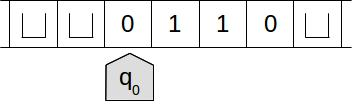
\includegraphics[scale=0.5]{TM}
\caption{\label{fig:Turing-Machine}Turing Machine}
\end{figure}

\begin{definition}[Turing Machine]
\label{def:Turing-Machine}
A \emph{Turing machine} is a 7-tuple $\left(Q,\Gamma,\sqcup,\Sigma,q_{i},q_{f},\tau\right)$ where:
\begin{align*}
 & Q \quad \text{is a finite, non-empty, set of \emph{states},} \index{Machine State} \\
 & \Gamma \quad \text{is a finite, non-empty, set of \emph{tape symbols},} \index{Tape Symbol} \\
 & \sqcup\in\Gamma \quad \text{is the \emph{blank symbol},} \index{Blank Symbol} \\
 & \Sigma\subseteq\Gamma\setminus\sqcup \quad \text{is the set of \emph{input symbols},}  \index{Input Symbol} \\
 & q_{o}\in Q \quad \text{is the \emph{initial state},} \index{Initial State} \\
 & q_{f}\in Q \setminus \{q_o\} \quad \text{is the \emph{final state},} \index{Final State} \\ 
 & \tau:\left(Q\setminus \{q_{f}\}\right)\times\Gamma \rightarrow  Q\times\Gamma\times\left\{ L,R,S\right\} \quad\text{is a partial \emph{transition function}. \index{Transition Function} }
\end{align*}
\end{definition}

The algorithm implemented by the machine is given by the transition function $\tau$. This function specifies that given the current state of the machine and the tape symbol under the head, the machine will reach a new state, will write a new symbol on tape (or leave the old symbol unchanged), and will move the head to the left, to the right, or stay in place ($L$, $R$ or $S$ respectively). After a finite, uniquely determined, succession of steps, the machine will reach the final state $q_f$ and \emph{halts} (the machine does not make any further move after halting). The output of the algorithm is the unique string of symbols $s \in \Sigma^\ast$  that is left on the tape after halting. Eventually, some machines could iterate forever, never halting. If an undefined transition is reached, the machine will get stalled.

The input to the machine is a string of symbols, and we assume that in the initial state the head of the machine is located at the first symbol of the input string. If we want to solve a problem related to an object $O$ other than a string, fist we have to provide a method to encode that object using a string $\left\langle O \right\rangle$.

\begin{example}
\label{ex:Turing-Machine}
The following Turing machine solves the problem of adding two natural numbers: the set of states is $Q = \left\{q_{o}, q_{1}, q_{f}\right\}$, the set of tape symbols is $\Gamma = \left\{0, 1, \sqcup \right\}$, the set of input symbols is $\mathcal{B} = \left\{0, 1 \right\}$, and the transition function is given by the following table (rows are indexed by machine states, and columns by tape symbols):

\begin{table}[h]
\centering
\begin{tabular}{l l l l}
\toprule
 & 0 & 1 & $\sqcup$ \\
\midrule
$q_{o}$ & $\left(q_{f}, \sqcup, S\right)$ & $\left(q_{1}, \sqcup, R\right)$ & $\uparrow$ \\
$q_{1}$ & $\left(q_{f}, 1     , S\right)$ & $\left(q_{f}, 1     , R\right)$ & $\uparrow$ \\
\bottomrule
\end{tabular}
\caption{Transition Rules}
\end{table}

Given the natural numbers $n$ and $m$, the input string for this machine is $n$ 1's followed by a $0$ and followed by $m$ 1's. The output is a string of $n+m$ consecutive 1's. For example, if we want to add the numbers 2 and 3 the input string should be $\sqcup 1 1 0 1 1 1 \sqcup$, and the machine output string would be $\sqcup 1 1 1 1 1 \sqcup$.
\end{example}

A Turing machine can be also represented by a \emph{state diagram}\index{State diagram}. A state diagram is similar to a labeled directed graph\footnote{In this particular case we allow loops and multiple edges coming out from vertices.} where the vertices are the states of the machine, the edges represent a movement from one state to another state, and the edge labels shows the symbol under the head that yields to the new state, together with the symbol written down in the tape and the movement of the head. Under these conventions, the state diagram of the Turing machine of Example \ref{ex:Turing-Machine} is depicted in Figure \ref{fig:Example-Turing-Machine}.

\begin{figure}[h]
\centering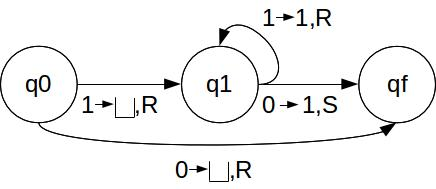
\includegraphics[scale=0.5]{ETM}
\caption{\label{fig:Example-Turing-Machine}Example of Turing Machine}
\end{figure}

It is a remarkable fact that small changes to the actual definition of Turing machine do not alter its power. That is, it is a highly robust definition. In Example \ref{ex:multitape_turing_machine} it is shown that adding more tapes to the machines does not increase the number of problems that can be solved using this model. Similar proofs can be provided for the case of adding a finite storage to the control tape, allowing parallel processing with multiple control heads, and so on.

\begin{example}
\label{ex:multitape_turing_machine}
A \emph{multitape Turing machine}\index{Multitape Turing machine} is a Turing machine that has multiple heads with their corresponding tapes. At the starting configuration the input string is in tape 1 and all the others tapes are blank. The transition function of a multitape Turing machine is:
\[
\tau:\left(Q \setminus q_{f} \right) \times \Gamma^k \rightarrow  Q \times \Gamma^k \times \left\{L,R,S\right\}^k.
\]
where $k$ is the number of tapes. Multitape Turing machines are equivalent to regular Turing machines. We can prove this assertion by providing a mechanism in which a regular Turing machine can simulate the behavior of a multitape machine. In order to do that we have to encode the content of the multiple tapes into a single tape, introducing a new symbol that will act as tape separator, and to codify the location of the heads in all those tapes, by means of a new head location symbol. If the tape separation symbol is $|$ and the head location symbol is $h$, a simulation tape of a 3-tapes machine could looks something like $\sqcup01h00|000h1|h0101\sqcup$. The operation of the regular machine just scans one by one the subtapes locating the head position and performing the required transition. If the computation of one subtape requires to write a new symbol beyond it limits, we have to shift the rest of the symbols to make room to the new symbol. Of course, the operation of the simulation will be much slower than the original multitape machine, but the set of problems that can be solved with the two types of machines is exactly the same.
\end{example}

Without any loss of generality, for the rest of this book we will assume that the set of input symbols $\Sigma = \mathcal{B}$ and that the set of tape symbols $\Gamma = \left\{0, 1, \sqcup \right\}$.

\begin{definition}\index{Configuration}
A \emph{configuration} of a Turing machine $T$ is the 3-tuple $\left(q,s,i\right)$, where $q\in Q$ is an state of the machine, $s\in\Gamma^+$ is a string with the contents of the tape (excluding the blank symbols), and $1 \le i \le n$ is the index of the symbol $s_i$ under the head, where $s_1$ is the first non-blank symbol of the tape and $n=l(s)$. 
\end{definition}

Configurations allow us to losslessly describe the current state of a Turing machine. At any step of a computation we could stop the machine, write down its current configuration, and later on continue the computation at the same point where we left, just by reading its configuration.

\begin{definition}\index{Configuration yields configuration}
We say that configuration $C=\left(q,s,i\right)$ \emph{yields} configuration $C'=\left(r,s',j\right)$ if there exists a transition $\tau:\left(q, s_{i}\right) = \left(r, s'_{i}, a\right)$, where $s=s_{1} \dots s_{i-1}s_{i}s_{i+1} \dots s_{n}$, $s'=s_{1} \dots s_{i-1}s'_{i}s_{i+1} \dots s_{n}$, and
\begin{equation}
  j = \begin{cases}
        i+1 & \text{if $a=R$} \\
        i-1 & \text{if $a=L$} \\
        i   & \text{if $a=S$}
  \end{cases}
\end{equation}
\end{definition}

Given the concepts of configuration and configuration that yields a new configuration we can formally define what we mean by computation.

\begin{definition}[Computation]\index{Computation}
Let $T$ be a Turing machine, $C_{0}$ the starting configuration of the machine, and $C_n$ a configuration containing the final state $q_f$. A \emph{computation} under machine $T$ is a finite sequence of $n+1$ configurations $\left(C_{0},C_{1},\ldots,C_n\right)$ in which each configuration $C_{k}$ yields the configuration $C_{k+1}$, for all $0\leq k < n$.
\end{definition}

Computations are deterministic, that is, given a Turing machine $T$ and an input string $s$, the sequence of configurations is predetermined. If the machine $T$ does not halt, or it get stalled, on input $s$, we say that there was no computation.

\begin{example}
The computation of the Turing machine described in Example \ref{ex:Turing-Machine} with the input string $110111$ is the following sequence of configurations:

\begin{enumerate}
\item $(q_0, 110111, 1)$
\item $(q_1, 10111,  1)$
\item $(q_1, 10111,  2)$  
\item $(q_f, 11111,  2)$  
\end{enumerate}

\end{example}

The next theorem states that our intuitive notion of computable procedure is equivalent to the concept of Turing machine. This result is not a regular theorem, since it cannot be formally proved. Some authors call it \emph{thesis} instead of theorem; Turing himself called it a \emph{definition}.

\begin{theorem}[Turing's Thesis]
\label{th:turing_thesis}
A procedure can be computed by a human being if, and only if, it can be computed by a Turing machine.
\end{theorem}

As we have mentioned in the introduction of this chapter, all the other alternative formalizations of the concept of computable procedure proposed so far are equivalent in expressive power to Turing machines. 

%
% Section: Universal Turing Machine
%

\section{Universal Turing Machines}
\label{sec:Universal-Turing-Machines}

In Section \ref{sec:Turing-Machines} we saw how to store the current state of a Turing machine so that the computation could be stopped and later on resumed. In Example \ref{ex:Encoding_TM} we are going to see a similar procedure, not to store the current state of the machine, but to save a full description of the machine itself. This procedure will allow us to enumerate, that is, to list all possible Turing machines. This enumeration will enable us to prove that there exists problems that are not solved by any Turing machine (see Section \ref{sec:non_computable_problems}), and to introduce the very important concept of \emph{Universal Turing Machine}.

\begin{example}
\label{ex:Encoding_TM}
In order to loosely describe a Turing machine we have to encode the transition function $\tau:\left(Q\setminus \{q_{f}\}\right)\times\Gamma\rightarrow Q\times\Gamma\times\left\{ L,R,S\right\}$. This function can be represented as a collection of quintuples $\left(q,s,r,t,a\right)$ where $q \in \left(Q\setminus \{q_{f}\}\right)$, $r \in Q$, $s$ and $t\in\Gamma$, and $a\in\left\{ L,R,S\right\}$. In this way, any Turing machine $T$ will be fully described by a collection of quintuples:
\[
\left(q_{1},s_{1},r_{1},t_{1},a_{1}\right),\left(q_{2},s_{2},r_{2},t_{2},a_{2}\right),\ldots,\left(q_{m},s_
{m},r_{m},t_{m},a_{m}\right)
\]
where $m \leq d\left(Q\setminus \{q_{f}\} \times d(\Gamma) \right)$, with the additional requirement that the first quintuple should refer to the initial state, and second one to the final state, that is $q_{1} = q_{o}$ and $r_{2} = q_{f}$. A possible description of these quituples would be to encode the elements of the set $Q\cup\Gamma\cup\left\{ L, R, S \right\}$ using a fixed length binary code (see Definition \ref{def:Fixed-Length-Codes} for more information about these codes), so the quintuple $\left(q,s,r,t,a\right)$ would be encoded as $\left\langle q, s, r, t, a \right\rangle$. The length of an encoded quintuple is $5l$, where $l=\left\lceil \log\left(d\left(Q\cup\Gamma\cup\left\{ L,R,S\right\} \right)\right)\right\rceil$. Using those conventions, the machine $T$ would be encoded as the binary string:
\[
\left\langle T \right\rangle = \left\langle \bar{l}, \left\langle q_{1}, r_{1}, s_{1}, t_{1}, a_{1} \right\rangle, \ldots, \left\langle q_{r}, r_{r}, s_{r}, t_{r}, a_{r} \right\rangle \right\rangle 
\]
The length of the encoded machine using this schema would be $l(\left\langle T \right\rangle) \leq 5lm + \log l + 1$.
\end{example}

Since each Turing machine is composed by a finite set of quintuples, we can encode and list all the machines using a shortlex ordering. We associate each machine $T$ with the index $i$ corresponding to its position in this list, and we denote by $T_i$ the i-th Turing machine. Each positive integer $i$ encodes one, and only one, Turing machine. However, as Proposition \ref{prop:padding_lemman} shows, all Turing machines have an infinite number of indexes. We associate each Turing machine with its smallest index.

\begin{proposition}[Padding Lemma]
\label{prop:padding_lemman}
Each Turing machine has infinitely many indexes.
\end{proposition}
\begin{proof}
If $T_i$ is the i-th Turing machine encoded by the string $\langle T_i \rangle$, we can add an finite number of 0's to the end of this string, resulting in a new encoding index $j$, that encodes the same machine.
\end{proof}

A universal Turing machine is a machine that can simulate the behavior of any other Turing machine on arbitrary input. The universal machine essentially achieves this by reading from its own tape both the description of the machine to be simulated (for instance, using the coding schema described in Example \ref{ex:Encoding_TM}), as well as the input string to be used during the computation.

\begin{definition}[Universal Turing Machine]
\label{def:Universal-Turing-Machine}
\index{Universal Turing machine}
A \emph{Universal Turing Machine} is a Turing machine $U$ such that $U(\langle \langle T_i\rangle, s \rangle) = T_i(s)$ for all Turing machines $T_i$ and all input strings $s \in \mathcal{B}$.
\end{definition}

Of course, we have to prove that such machine exits before we can use it. We could argue that a human being would be able to decode the machine $T_i$ and simulate its behavior with the input string $s$, and then refer to Theorem \ref{th:turing_thesis}. A better approach would be to explicitly build an universal Turing machine. However, describing one of these machines is out of the scope of this book. Instead, we refer to the reader to the references included at the end of the chapter.

%
% Section: Non computable problems
%

\section{Non-Computable Problems}
\label{sec:non_computable_problems}

Turing machines allow us to identify which problems can be solved using effective procedures, that is, the set of problems that can be worked out with computers. Although it might be a bit surprising, there exists many problems that cannot be solved using algorithms. These problems are beyond the capabilities of computers. We are not talking about problems like if a computer can be intelligent or if it can be self-aware, we refer to well defined mathematical problems. For example, the famous \emph{halting problem} asks to find a computer program that, given any other program and an input string, decides if the program will eventually stop for that input string, or if it will keep running forever.

\begin{algorithm}
\caption{HALT function}
\label{alg:halt}
\begin{algorithmic}
\Procedure{HALT}{$A, I$}
    \If{$A(I)$ halts} 
        \State \textbf{return} $1$
    \Else
        \State \textbf{return} $0$
    \EndIf
\EndProcedure
\end{algorithmic}
\end{algorithm}

\begin{theorem}[Halting Problem]
\index{Halting problem}
\label{th:halting-problem}
Define the HALT as in Algorithm \ref{alg:halt}. It does not exists a Turing machine that computes the $HALT$ function for all possible pairs $(A, I)$, where $A$ is a Turing machine and $I$ is the input string to that machine.
\end{theorem}
\begin{proof}
The proof is by contradiction. Assume that the machine $HALT$  exists, and define a new Turing machine $TC$ such that $TC(A) = 1$ if $HALT(A,A) = 0$, and $TC(A)$ will never stop if $HALT(A,A) = 1$. Then the contradiction arises when we ask about the result of $TC(TC)$: if $TC(TC)$ stops we have that $HALT(TC,TC) = 0$ and that $TC(TC)$ should not stop, and if $TC(TC)$ does not stop then we have that $H(TC,TC) = 1$ and thus $TC(TC)$ should stop.
\end{proof}

A very important consequence of the Halting Problem is that there exists more well-defined mathematical problems than computable solutions\footnote{It is still an open question if there exists non-computable problems in Nature.}. The Halting Problem has also important practical consequences in computer programming. For example, we cannot write a program that can guarantee that any other arbitrary program is bug-free, or that all infinite loops with conditional exits will eventually stop for all possible inputs.

Incomputability is not only about halting. Next example shows a well defined practical problem involving simple strings manipulation that can not be solved using computers.

\begin{example}
\label{ex:PCP}
Given two finite lists $\left( \alpha_1, \ldots, \alpha_n \right)$ and $\left( \beta_1, \ldots, \beta_n \right)$ of strings over some alphabet $\Sigma$, where $d(\Sigma) \ge 2$, the \emph{Post Correspondence Problem}, or PCP, asks to decide if there exists a sequence of $K \geq 1$ indices $(i_k)$, where $1 \le i_k \le n$ for all $1 \le k \le K$, such that $\alpha_{i_1} \ldots \alpha_{i_K} = \beta_{i_1} \ldots \beta_{i_K}$. For example, given the sequences $(a, ab, bba)$ and $(baa, aa, bb)$, a solution to the problem would be $\alpha_3 \alpha_2 \alpha_3 \alpha_1 = \beta_{3} \beta_{2} \beta_{3} \beta_{1}$. It does not exist an algorithm to solve PCP. As many proofs of incomputability, the proof proceed by showing that HALT can be reduced to PCP, that is, if PCP is decidable then the Halting problem should be decidable as well. We are not going to show the details of the proof in this section. For the interested reader, we refer to the references at the end of this chapter.
\end{example}

%
% Section: Computable Functions and Sets
%

\section{Computable Functions and Sets}
\label{sec:computable_functions}

Each Turing machine $T$ defines a function $f_T:\mathcal{B}^{\ast}\rightarrow\mathcal{B}^{\ast}$ in such a way that for each input string $s\in\mathcal{B}^{\ast}$ assigns the output string $T(s)\in\mathcal{B}^{\ast}$. This relation between Turing machines and functions allows us to introduce the concept of \emph{computable function}. 

\begin{definition}
\label{def:computable-function}
\index{Computable Function}
A function $f:\mathcal{B}^{\ast}\rightarrow\mathcal{B}^{\ast}$ is \emph{computable} is there exist a Turing machine $T$ such that it defines the function $f$.
\end{definition}

Computable functions are also called \emph{recursive functions}. However, since we are not going to cover the theory of recursive functions in this book, we prefer the term computable functions.

\begin{example}
The function that assigns to each pair of natural numbers $x$ and $y$ its sum $x + y$ is a computable function, as it is shown in Example \ref{ex:Turing-Machine}. In this particular case, we have transformed the original function $f: \mathbb{N} \times \mathbb{N} \rightarrow \mathbb{N}$ into a new function $g:\mathcal{B}^{\ast}\rightarrow\mathcal{B}^{\ast}$ by means of encoding natural numbers as strings of 1's, and the pair of numbers $x$, $y$ into a single string $\left\langle x, y \right\rangle$.
\end{example}

Partial functions can be defined by Turing machines that do not halt on the undefined values of the function.

\begin{definition}
A partial function $f:\mathcal{B}^{\ast}\rightarrow\mathcal{B}^{\ast}$ is \emph{partial computable} is there exist a Turing machine $T$ such that it defines the function $f$ for those values in which $f$ is defined, and $T$ does not halt for those values in which $f$ is not defined.
\end{definition}

\begin{example}
The function $f: \mathbb{N} \times \mathbb{N} \rightarrow \mathbb{N}$ that assigns to each pair of natural numbers $x$ and $y$ the number $x - y$ is a partial computable function, since it is not defined in the case that $x < y$.
\end{example}

We can apply the same concepts of computable and partial computable to sets.

\begin{definition}
A set $A \in \mathcal{B}^\ast$ is \emph{computable} if its characteristic function $\mathcal{X}_A$ is a total computable function. A set $A \in \mathcal{B}^\ast$ is \emph{computably enumerable} if its characteristic function $\mathcal{X}_A$ is a partial computable function, that is, $\mathcal{X}_A(a) = 1$ if $a \in A$, but $\mathcal{X}_A(a)$ is undefined if $a \not\in A$.
\end{definition}

\begin{example}
The set of all Turing machines that halt on all inputs is not computable, as we have shown in Theorem \ref{th:halting-problem}, although it is computably enumerable.
\end{example}

{\color{red} TODO: Introduce the concept of reducibility.}

%
% Section: Oracle Turing Machine
%

\section{Oracle Turing Machine}
\label{sec:oracle_turing_machine}

{\color{red} TODO: Introduce the concept}

{\color{red} TODO: Provide a diagram}

Withe the aid of the Oracle, a Turing machine could solve uncomputable problems, like the halting problem.

{\color{red} The oracle tape is a one-way unbounded, read-only tape that contains all the values of the characteristic function $\chi_\mathcal{O}$. We assume that it takes, for arbitrary $w \in \Sigma^\ast$, only one step to search the tape and return the value of $\chi_\mathcal{O}(w)$.}

\begin{definition}[Oracle Turing Machine]
\label{def:Oracle-Turing-Machine}
An \emph{oracle Turing machine} with oracle set $\mathcal{O}$ is a 8-tuple $\left(Q, \Gamma, \sqcup, \Sigma, q_i, q_f, \tau, \mathcal{O} \right)$ where:
\begin{align*}
 & Q \quad \text{is a finite, non-empty, set of \emph{states},} \index{Machine State} \\
 & \Gamma \quad \text{is a finite, non-empty, set of \emph{tape symbols},} \index{Tape Symbol} \\
 & \sqcup\in\Gamma \quad \text{is the \emph{blank symbol},} \index{Blank Symbol} \\
 & \Sigma\subseteq\Gamma\setminus\sqcup \quad \text{is the set of \emph{input symbols},}  \index{Input Symbol} \\
 & q_{o}\in Q \quad \text{is the \emph{initial state},} \index{Initial State} \\
 & q_{f}\in Q \setminus \{q_o\} \quad \text{is the \emph{final state},} \index{Final State} \\ 
 & \tau: \left(Q \setminus \{q_{f}\}\right) \times \Gamma \times \{0, 1\} \rightarrow  Q\times\Gamma\times\left\{ L,R,S\right\} \quad\text{is the \emph{transition function}, \index{Transition Function} } \\
 & \mathcal{O} \subseteq \Sigma^\ast \quad \text{is the \emph{oracle set}.}
\end{align*}
\end{definition}

Properties:

 * The machine is independent of the oracle set
 * Turing machines are a subset of oracle Turing machines

Talk about:

 * How to encode oracle Turing machines
 * What means a function or set to be oracle computable
 * 

%
% Section: Computational Complexity
%

\section{Computational Complexity}
\label{sec:computational_complexity}

{\color{red} Computational Complexity theory is an investigation of the time, memory, or other resources required for solving computational problems.} In this book we are insterested mostly in the time required to solve a problem. {\color{red} We compute the running time of an algorithm as a function of the length of the string representing the input.}

{\color{red} TODO: Adapt this definiton.}
\begin{definition}
Let $M$ a deterministic Turing machine that halts on all inputs. The running time or time complexity of $M$ is the function $f:\mathbb{N}\rightarrow\mathbb{N}$, where $f(n)$ is the maximum number of steps that $M$ uses in any input of length $n$. If $f(n)$ is the running time of $M$, we say that $M$ runs in time $f(n)$ and that $M$ is an $f(n)$ time Turing machine.
\end{definition}

{\color{red} It considers only the highest order term of the expression for the running time of the algorithm, disregarding both the coefficient of that term and any lower order terms.}

{\color{red} Introduce polynomial bounds $O(n^c)$}

{\color{red} TODO: Adapt this definiton.}
Let $t:\mathbb{N}\rightarrow\mathbb{R}^{+}$ be a function. Define the time complexity class, $TIME(t(n))$, to be the collection of all languages that are decidible by an $O(t(n))$ time Turing machine.

{\color{red} TODO: Add the following as an example:
Let $t(n)$ be a function, where $t(n)\geq n$. Then every $t(n)$ time multiple tape Turing machine has an equivalent $O(t^{2}(n))$ time single-tape Turing machine.
}

{\color{red} Polynomial differences in running time are considered to be small, whereas exponential differeces are considered to be large.}


{\color{red} Adapt this definition:
\begin{definition}
$P$ is the class of languages that are decidible in polynomial time on a deterministic single-tape Turing machine $P=\cup_{k}TIME(n^{k})$.
\end{definition} 

$P$ roughly corresponds to the class of problems that are realistically solvable on a computer.}

{\color{red} Add the following example of problem in P: PATH = \{ $\langle G,s,t\rangle|G$ is a directed graph that has directed path from $s$ to $t$ }

{\color{red} Adapt this definition:
\begin{definition}
A verifier for a language $A$ is an algorithm $V$, where $A=\{w|V$ accepts $\langle w, c\rangle$ for some string $c\}$.
\end{definition}
}

{\color{red} We measure the time of a verier only in terms of the length of $w$, so a polynomial time verifier runs in polynomial time in the length of $w$
. A language $A$ is polynomially verifiable if it has a polynomial time verifier. The symbol $c$ is called a certificate, or proof of membership in $A$.}

{\color{red}
\begin{definition}
$NP$ is the class of languages that have polynomial time verifiers.
\end{definition}
}


{\color{red} TODO: Include an example.}

{\color{red} $P$ is the class of languages for which membership can be decided quickly. $NP$ is the class of languages for which membership can be verified quickly. The question of whether $P=NP$ is one of the greatest unsolved problems in theoretical computer science and contemporary mathematics.}


{\color{red} TODO: Not sure about the rest of this chapter:

Definition 14. A function $f:\Sigma^{\ast}\rightarrow\Sigma^{\ast}$ is a polynomial time computable function if some polynomial time Turing machine $M$ exists that halts with just $f(w)$ on its tape, when started on any imput $w$.

When problem $A$ reduces to problem $B$, a solution to $B$ can be used to solve $A$.

Definition 15. Language $A$ is polynomial time mapping reducible, or simply polynomial time reducible, to language $B$, written $A\leq_{P}B$, if a polynomial time computable function $f:\Sigma^{\ast}\rightarrow\Sigma^{\ast}$ exists, where for every $w$ $w\in A\iff f(w)\in B$

The function $f$ is called the polynomial time reduction of $A$ to $B$.

If one language is polynomial time reducible to a language already known to have a polynomial time solution, we obtain a polynomial time solution to the original language.

Theorem 16. If $A\leq_{P}B$ and $B\in P$, then $A\in P$.

Definition 17. A language $B$ is NP-complete if it satisfies two conditions: $B$ is in $NP$, and every $A$ in $NP$ is polynomial time reducible to $B$.

Theorem 18. If $B$ is NP-complete and $B\in P$, then $P=NP$.

Theorem 19. If $B$ is NP-complete and $B\leq_{P}C$ for $C$ in $NP$, then $C$ is NP-Complete.

}

%
% Section: References
%

\section*{References}

The original paper form Alan Turing where the concepts of Turing machine, universal Turing machine, and non-computable problems were introduced is \cite{turing1936computable}, however it is a difficult to read paper for the contemporary reader. An easier to read introduction to computability theory, from the point of view of languages, can be found in \cite{sipser2012introduction}, and a more advanced introductions in \cite{cooper2003computability} and \cite{soare2016turing}. In \cite{fernandez2009models} we can find a description of the most important computability models proposed so far. The Post Correspondence Problem was introduced by Emil Post in \cite{post1946variant}; for the details of the proof sketched in Example \ref{ex:PCP} please refer to \cite{sipser2012introduction}.

{\color{red} TODO: Add a reference to how to build a universal Turing machine.}

